\documentclass[12pt,a4paper]{report}
\usepackage{graphicx}
\usepackage{hyperref}
\usepackage[all]{hypcap}
\usepackage{times}
\usepackage{xcolor}
\usepackage{tabulary}
\usepackage[top=3cm, bottom=3cm, left=3cm, right=2cm]{geometry}
\hypersetup{
    pdftoolbar=true,        % show Acrobat’s toolbar?
    pdfmenubar=true,        % show Acrobat’s menu?
    pdffitwindow=false,     % window fit to page when opened
    pdfstartview={FitH},    % fits the width of the page to the window
    pdftitle={Report of building a wireless communication system},    % title
    pdfsubject={Report},   % subject of the document
    colorlinks,
    linkcolor=violet,
    citecolor=blue,
    urlcolor=brown
}

\begin{document}
    \title{Report of building a wireless communication system}

    \author{course code: B30SQ \\ by Yifei Jing, Xunyu Kai, Zhi Chai}
    \date{April, 2020}
    \maketitle
    \setlength\parindent{0pt}

\chapter*{Introduction}
The aim of this project is to build a wireless communication system based on what is learn in the course \emph{B30SQ}.
The structure of a communication system is depicted in \hyperref[fig:system_structure]{Figure \ref*{fig:system_structure}}, which composes of a transmitter and a receiver between two computers.
The transmitter composes of a modulator, a frequency converter, an amplifier, and a patch antenna. The receiver includes a patch antenna, an amplifier, a frequency converter, and a demodulator.
In this project, the modulator is implemented using an integrated USB TTL converter, which simply transform the sequence of 0s and 1s from the computer onto electric signal with 0V indicating 0, and 3.3V indicating 1. The frequency converter is achieved using the integrated module.
The amplifiers contain the Low Noise amplifier designed as the first component to the receiver, the op-amps to provide the second level signal amplification at the receiver and the power amplification at the transmitter.
The type of the antenna is the patch antenna, as the principle is easy to be understood. The frequency converter at the receiver end is implemented using a low pass filer.

For the choice of the frequency band, 2400Mhz-2500Mhz is chosen according to ISM: Frequency bands designated for Industrial, Scientific and Medical use.

\begin{figure}[ht]
    \centerline{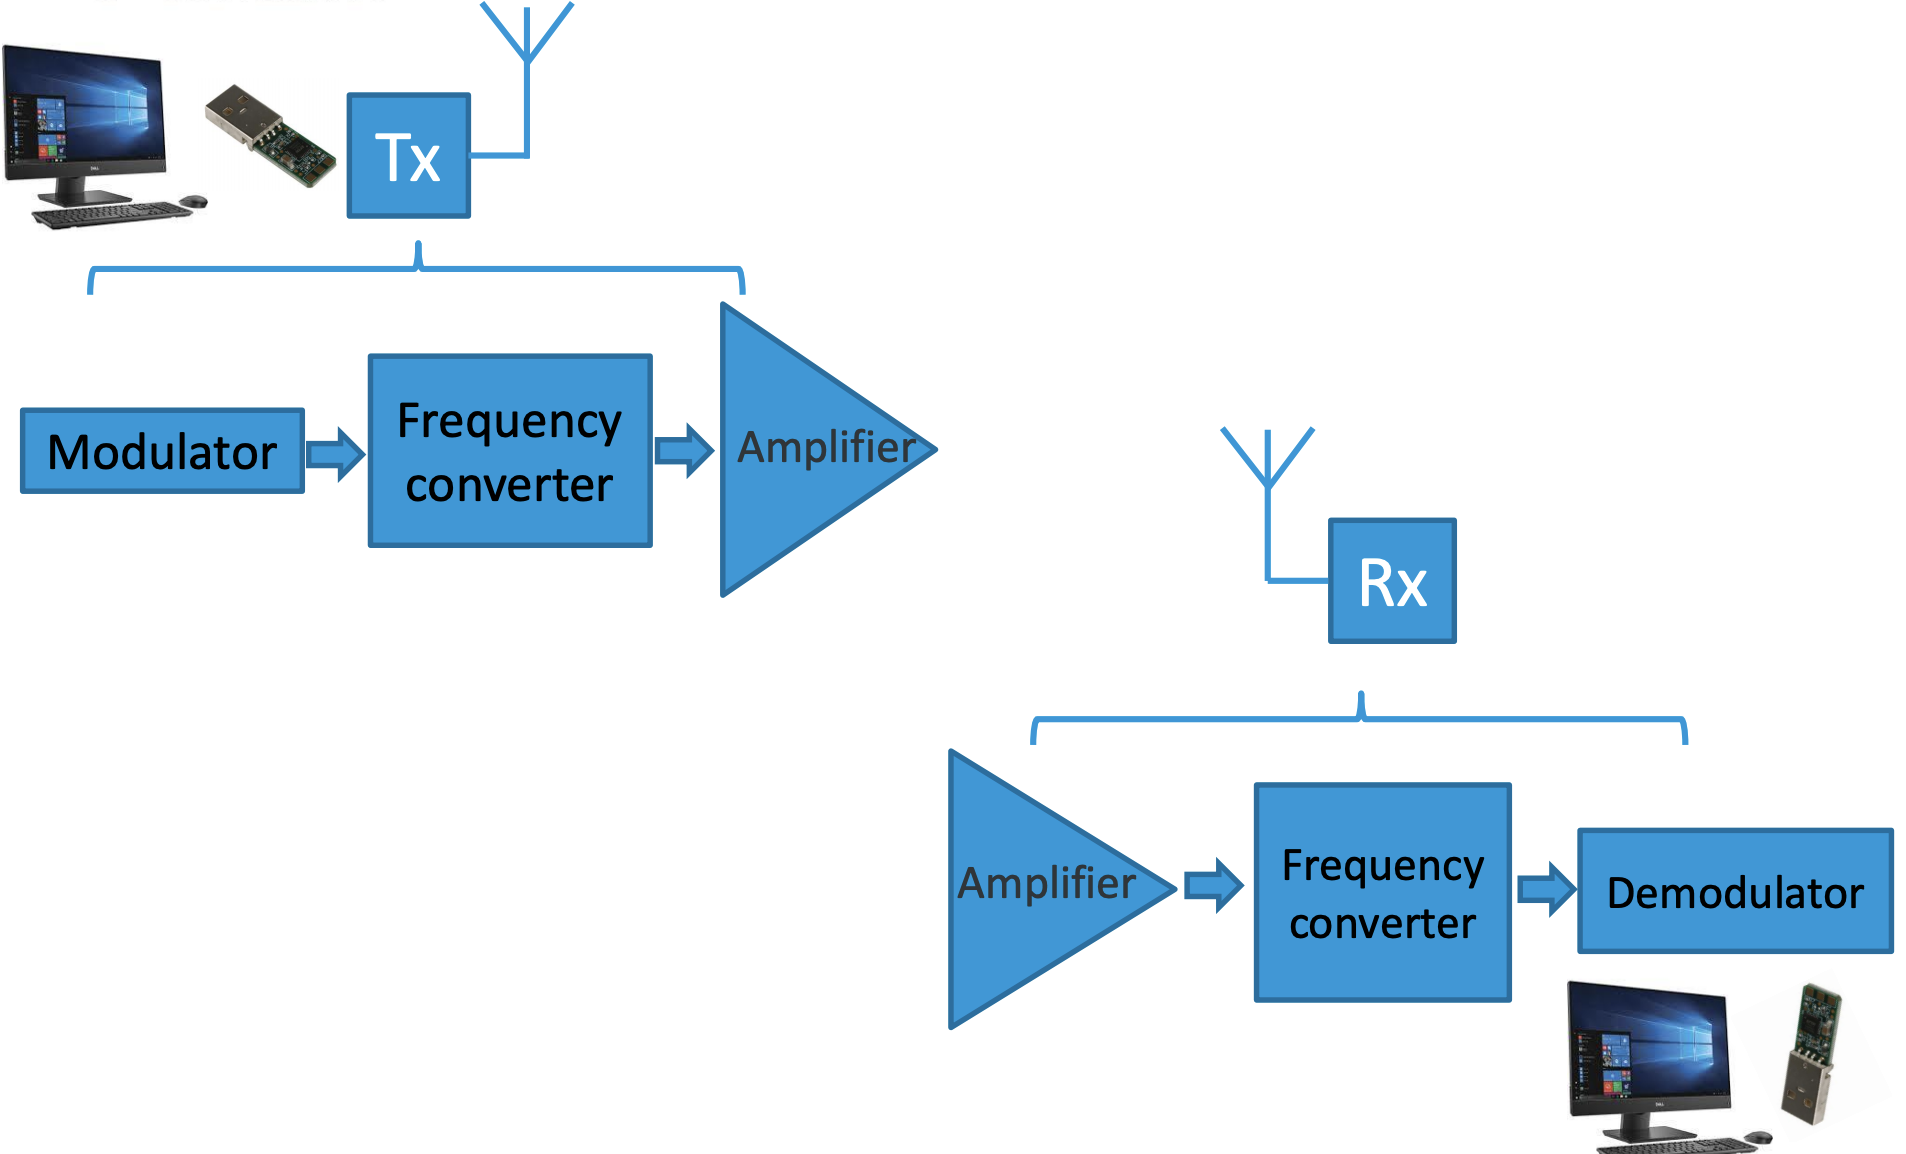
\includegraphics[scale=1]{system_structure}}
    \caption{The structure of a communication system}
    \label{fig:system_structure}
\end{figure}

\chapter*{Patch antenna design}
\chapter*{Amplifier design}
\chapter*{Transmitter's modulator}
\chapter*{Entire system testing}

    
\end{document}